\documentclass[10pt,a4paper]{article}
\usepackage[utf8]{inputenc}
\usepackage{amsmath}
\usepackage{amsfonts}
\usepackage{amssymb}
\usepackage{graphicx}
\usepackage{fullpage}

\newenvironment{boxed2}
    {\begin{center}
    \begin{tabular}{|p{\textwidth}|}
    \hline \\
    }
    { 
    \\ \\ \hline
    \end{tabular} 
    \end{center}
    }


\begin{document}
\section{Introduction}



\section{Graph Neural Networks}
Neural networks are a class of universal function approximators, composed layer-wise by functions $\mathcal{L}^1\circ\mathcal{L}^2\circ ... \circ \mathcal{L}^n $, where each layer-to-layer transition map $\mathcal{L}^i$ is a trainable function from some feature space associated with layer $L$ to a feature space associated with layer $L+1$.

Many modern approaches use a specific type of neural network, referred to as a Graph Neural Network (GNN), which act on data encoded in features associated with some representative graph (i.e. a collection of nodes and connections between them).


%\section{Group Representations, Equivariance, and Invariance}
A group $G$ is a set with a binary, associative product defined between it's elements under which it is closed, and for which every element, there exists an inverse element (and which also contains an identity element).



%\subsubsection*{Matrix Representations of Groups}
A matrix representation $\mathcal{D}_{V}$ of a group $G$ is a map from elements of $G$ to square matrices such that for all elements $g,h\in G$, there are representations satisfying:
$$
\mathcal{D}(g)\mathcal{D}(h)=\mathcal{D}(gh)
$$
Note that we often discard the 'matrix' from 'matrix representation' and often refer only to representations of groups, though these are synonymous for our purposes here.


%\subsubsection*{Equivariance}
A function $f:X\rightarrow Y$ is equivariant with respect to a group $G$ if, for representations $\mathcal{D}_X$ and $\mathcal{D}_Y$ of $G$ (over spaces $X$ and $Y$, respectively), it satisfies:
$$
f(D_X(g)x) = D_Y(g)f(x) \quad\quad \forall g\in G
$$
Essentially, a function is equivariant with respect to some group if it 'commutes' with the representations of groups on it's input and output space. 

%\subsubsection*{Invariance}
A special case of equivariance then is \textit{invariance}, where the representations of all group elements in the output space are identity (i.e. $D_Y$ is the trivial representation). That is, a function $f:X\rightarrow Y$ is invariant under a group $G$ if it satisfies:
$$
f\circ \mathcal{D}_X(g) = f \quad
\ \forall g\in G.
$$




%\section{$SO(3)$ Equivariant Networks}
In the case of $SO(3)$, representations over a vector space of dimension $2\ell+1$ are Wigner-$\mathcal{D}^{\ell}$ matrices. Thus, we define an $SO(3)$ equivariant network to be a neural network $f:H_1 \rightarrow H_2$, with domain $H_1:\lbrace h_{(\ell_1)}\rbrace$ and codomain $H_2:\lbrace h'_{(\ell_2)}\rbrace$ (both being direct products of harmonic tensor spaces), that satisfies:
$$
f(\lbrace \mathcal{D}^{\ell_1}(R)h_{(\ell_1)}\rbrace) = \lbrace\mathcal{D}^{\ell_2}(R) h'_{(\ell_2)}\rbrace \quad\quad \forall R\in SO(3)
$$
The harmonic components $h_{\ell}^m$ (where $h_{\ell}$ generally refers to a $2\ell+1$ dimensional vector) correspond most naturally to the coefficients of spherical harmonic tensors, and in the context of machine learning, act as a feature space for data.

\subsection{Representation/Feature Space}
In an $SO(3)$-network, features are generally associated with irreducible representations of groups. In the case of $SO(3)$, these irreducible representations are spherical harmonics $Y_{\ell}^m$, indexed by two sets, the rotational order $\ell\geq 0$, and the azimuthal order $-\ell\leq m \leq \ell$.

Thus, a traditional feature set $V^{(n)a}$ of channel $a$ and associated with object $n$, has an additional two indices $\ell$ and $m$ in an $SO(3)$ network, corresponding to the aformentioned indices of a harmonic expansion.


\subsection{Layers}
Compositions of equivariant functions are themselves equivariant functions. As such, we may form an equivariant network by composing it layer-wise from a set of common equivariant functions.

Here, we consider three types of $SO(3)$-equivariant functions from which we may compose our equivariant networks: namely, $SO(3)$-feature convolutions, $\ell$-wise self-interactions and non-linearities, and pooling. An overview of each is given below.

\subsubsection{$SO(3)$ Convolution}
To maintain equivariance, for an input feature set of the type described above,  through convolution with some filter $F$,  the filter also must be associated with a set of spherical harmonics, and thus also has an additional two indices $\ell_f$ and $m_f$. 

Note here that the tensor product of two representation spaces is equivariant under transformation of the two subspaces, i.e.:
$$
\mathcal{D}^V\otimes \mathcal{D}^W=\mathcal{D}^{V\otimes W}
$$
Tensors products of $SO(3)$ representations are cleanly related to a third set of $SO(3)$ representations by way of Clebsch-Gordan coefficients $c^{\ell_3m_3}_{\ell_1m_1\ell_2m_2}$ as:
$$
(u\otimes v)_{\ell_o}^{m_o} = c_{\ell_1m_1\ell_2m_2}^{\ell_om_o}u_{\ell_1}^{m_1}v_{\ell_2}^{m_2}
$$
where $u$ and $v$ are harmonic vectors of order $\ell_1$ and $\ell_2$, respectively.

Thus, we maintain equivariance by defining convolution to be the scaled tensor product of the two representation spaces (i.e. that of the input feature space, and the filter space), so that layer to layer convolutional maps $\mathcal{L}$ may be defined component-wise as:
$$
\mathcal{L}^{\ell_o}_{acm_o}\big(\vec{r}_a,V_{acm_i}^{\ell_i}\big) = \sum_{m_f,m_i}c_{\ell_im_i\ell_fm_f}^{\ell_o m_o}\sum_{b}F^{\ell_f\ell_i}_{cm_f}(r_{ab})V_{bcm_i}^{\ell_i}
$$
where the filter function $F^{\ell_f\ell_i}_{cm_f}(r_{ab})$ depends only on the distance between point $a$ and $b$ (as opposed to directional dependence, to maintain equivariance), but has independent, trainable parameters for different rotational orders $\ell_f, \ell_i$, azimuthal orders $m$, and channels $c$.

\subsubsection{Self-Interaction}
Feature sets for individual objects may also update according to themselves as long as they act across $m$ for every $\ell$ and only update accordign to the different channels $c$. That is, functions of the form:
$$
V_{acm}^{\ell} \rightarrow  \sum _{c}W^{\ell}_{c'c}V_{acm}^{\ell}
$$
are also equivariant. 

\subsubsection{Non-Linearities}
We can also apply point-wise non linearities and maintain equivariance, as long as they also respect the across $m$ indices for every order feature $\ell$.

\subsubsection{Pooling}
Pooling, or aggregation, across all elements or objects (index $a$) while preserving the $m$ and $\ell$ indices is itself equivariant. Thus, functions of the form:
$$
 M_{cm}^{\ell} = \text{AGG}_{a}(\lbrace V_{acm}^{\ell}\rbrace)
$$ 
where $\text{AGG}$ is an arbitrary aggregation function performed only over the object index $a$, are also available in the construction of $SO(3)$ networks.

\subsection{Predicting Tensorial Data with SO(3) Networks}
Such $SO(3)$ equivariant networks are naturally well suited for the prediction of tensorial properties. Tensors may generally be decomposed into a set of $SO(3)$ invariant subspaces which can then each be associated with a set of spherical harmonics (see spherical harmonic decomposition of a tensor).

\subsubsection{Feature Pathways}
It should be clear that, from our definition of $SO(3)$ equivariant convolution, different order $\ell$ representations in the output space $V^{(L), \ell}_{acm}$ of final layer $L$, will be the result of interactions with potentially different $\ell_f$ order filters and the input layer features of order $\ell_i$. We here term the set of filter orders through the layers that result in a final output feature of order $\ell_o$ to be the \textit{feature pathway} of feature order $\ell_o$.

This feature pathway depends most generally on the chosen input feature orders $\ell_i$, as well as the order of the filters  $\ell_f$ for each layer, and the total number of layers. The pathway then may be determined by the selection rules of Clebsch-Gordon coefficients. That is, CG coefficients $c^{LM}_{\ell_1m_2\ell_2m_2}$ can only be non-zero when the following hold for some set of inputs $\ell_1,m_1$ and $\ell_2, m_2$:
\begin{itemize}
\item $M=m_1+m_2$
\item $|\ell_1-\ell_2|\leq L\leq \ell_1+\ell_2$
\end{itemize}
Thus, we may determine what filter orders $\ell_f$ contribute to some output of order $\ell_o$ of some network, for an input of order $\ell_i$.

Feature pathways are particularly relevant in the case of tensorial multi-target training sets, or transfer-learning applications, where different targets have different rotational order decompositions. In such cases, the filters learned for different datasets may not overlap at all, and thus would have disjoint feature pathways. 

For example, consider one layer of $SO(3)$ convolution, with input features of order $\ell_i=0,1$ and filters of order $\ell_f = 0,1,2$. The outputs of order $\ell_{o}=1$ would depend only on the trained parameters in filters of orders $\ell_i,\ell_f = (0,1),(1,0)$, whereas the outputs of order $\ell_{o}=2$ would depend only on filters of $\ell_i,\ell_f = (0,2),(1,1)$. 
\begin{center}
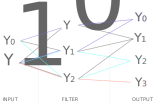
\includegraphics[scale=0.5]{featurepath_ex_12.pdf}
\end{center}
So, if a network was trained on a tensorial target set with a decomposition of order $\ell_o=2$ (i.e. a rank-two symmetric, traceless tensor), and then transfered and trained on a tensorial target of order $\ell_o = 3$ (i.e. a symmetric, traceless rank-3 tensor), there would only be overlap in the training of the $\ell_f=1$ filter weights.

 

%%%%%%%%%%%%%%%%%%%%%%%%%%%%%%%%%%%%%%%%%%%%%%%%
%%%%%%%%%%%%%%%%%%%%%%%%%%%%%%%%%%%%%%%%%%%%%%%%
%%%%%%%%%%%%%%%%%%%%%%%%%%%%%%%%%%%%%%%%%%%%%%%%
%%%%%%%%%%%%%%%%%%%%%%%%%%%%%%%%%%%%%%%%%%%%%%%%
%%%%%%%%%%%%%%%%%%%%%%%%%%%%%%%%%%%%%%%%%%%%%%%%
%%%%%%%%%%%%%%%%%%%%%%%%%%%%%%%%%%%%%%%%%%%%%%%%
%%%%%%%%%%%%%%%%%%%%%%%%%%%%%%%%%%%%%%%%%%%%%%%%
%%%%%%%%%%%%%%%%%%%%%%%%%%%%%%%%%%%%%%%%%%%%%%%%
%%%%%%%%%%%%%%%%%%%%%%%%%%%%%%%%%%%%%%%%%%%%%%%%
%%%%%%%%%%%%%%%%%%%%%%%%%%%%%%%%%%%%%%%%%%%%%%%%
%%%%%%%%%%%%%%%%%%%%%%%%%%%%%%%%%%%%%%%%%%%%%%%%
%%%%%%%%%%%%%%%%%%%%%%%%%%%%%%%%%%%%%%%%%%%%%%%%

\section{Spherical Harmonic Decomposition of a Tensor}
A spherical harmonic decomposition of a tensor is a partitioning of a tensor space into a set of disjoint harmonic subspaces $\mathcal{H}^{(\ell)}$ that are invariant under the special orthogonal group $SO(3)$. That is, for a tensor $T$ of rank $n$ (over the vector space ), a spherical harmonic decomposition of $T$ refers to a set $\lbrace h^{\ell}\rbrace$ of harmonic components where $0\leq \ell\leq n$; such that for transformations of $T$ under $R\in SO(3)$ (taking $\hat{e}_i\rightarrow R^i_{i'}\hat{e}_i$) with contravariant components transforming as:
$$
T_{x_1x_2...x_n}\rightarrow T_{x'_1x'_2...x_n'}=R_{x_1'}^{x_1} R_{x_2'}^{x_2} R_{x_3'}^{x_3}T_{x_1x_2...x_n},
$$
the harmonic subspaces remain invariant and transform as:
$$
\lbrace h^{(\ell)}\rbrace \rightarrow \lbrace h'^{(\ell)}\rbrace = \lbrace \mathcal{D}^{\ell}(R) h^{(\ell)}\rbrace
$$
where $\mathcal{D}^{\ell}(R)$ is the $\ell$-th order Wigner-$\mathcal{D}$ matrix representation of the transformation $R$, and $h^{(\ell)}$ represents a $(2\ell +1)$-dimensional vector  $[h_{\ell}^{-\ell},h_{\ell}^{-\ell+1},... h_{\ell}^{\ell}]$, with $h_{\ell}^{m}$ as coefficients of tensor spherical harmonics $Y_{\ell}^m$.

\subsection{Constructing $SO(3)$ Invariant Subspaces}
An invariant subspace of a tensor is a subspace which is closed under the action of some group of transformations. That is, invariant and disjoint subspaces of a tensor shouldn't 'mix' at all under the corresponding group transformations. 

Invariants under $SO(3)$ of an arbitrary tensor $T$ may be constructed by way of Young symmetrizers, and subsequent contractions with the metric tensor $g_{ij}$ or the fully antisymmetric tensor $\epsilon_{ijk}$. Note that these three methods correspond to the decomposition of a tensor with respect to the general linear group (by way of Young symmetrizers), the orthongonal group (contractions with $g_{ij}$), and the special linear group (contractions with $\epsilon_{ijk}$), respectively. 

Since $SO(3) =   SL(3)\bigcap O(3) \subset GL(3) $, to construct invariants of $SO$, we generally form invariant subspaces under $GL$ by way of Young symmetrizers first, and then construct invariants under $O$ and/or $SL$ of these $GL$ invariant subspaces. This often results in several different harmonic subspaces of the same order $\ell$  in the harmonic decomposition of a tensor.
Also, note that the $GL$ decompositions for tensors of rank greater than two are not, in general, unique.

Below, we introduce the tools used in the construction of such invariant subspaces and demonstrate their invariance. These tools are then applied in three cases of tensor spaces with importance in the field of materials science: corresponding to the space of dielectric tensors, piezoelectric response tensors, and elasticity tensors.

\subsubsection{$GL$ Decompositions}
By way of the Schur-Weyl duality, the invariant subspaces of a tensor under the general linear group $GL$ determine the invariant subspaces of the tensor under the symmetric group $S_n$, where symmetric group elements act as permutations on tensor indices.



Under the symmetric group, the invariant subspaces of a tensor are described by way of standard Young tableaux, and then constructed from an arbitrary tensor by means of the corresponding Young symmetrizers. Below, these concepts are briefly introduced for the purpose of $GL$ decompositions of tensors over $\mathbb{C}^n$. Note that these decompositions are in general not unique for tensors of rank $>2$, so some conventions must be adopted.

\begin{boxed2}
\textbf{Schur-Weyl Duality:}

\medskip

Under the joint action of the symmetric group $S_k$ and $GL_n$ acting on a tensor of rank-$k$ over $(\mathbb{C}^n)^{\otimes k}$, the tensor space may be decomposed into a direct sum of tensor products of representations of $S_k$, $\pi_k$ and representations of $GL_n$, here $\rho_n$, simultaneously indexed by the set of Young diagrams $\lambda$ of order $k$. That is,
$$
\underbrace{\mathbb{C}^n\otimes ... \otimes\mathbb{C}^n}_k= \bigoplus_{\lambda}\pi^{(\lambda)}_{k}\otimes\rho_n^{(\lambda)}.
$$
This is a statement of the Schur-Weyl duality without proof. The point here though is that the representations under $GL$ of a complex tensor product space, are indexed by the same set (that is, they both are described by the same underlying structure) as the representations under $S$.  Thus, we consider the $GL$ decomposition to be synonymous here with the symmetric group $S$ decomposition.
\end{boxed2}

\subsubsection*{Young Diagrams, Tableaux, and Symmetrizers}
Young diagrams of order $n$ are left-justified arrangements of boxes into $k$ rows stacked vertically in non-increasing order. 
\begin{figure}\centering

\includegraphics[scale=0.6]{youngdiagram-ex.pdf}
\caption{Example Young diagram of shape $(5,4,3,1)$.}
\end{figure}
A Young diagram is said to be of some shape $\lambda:(\lambda_1,\lambda_2,...,\lambda_k)$, where $\lambda_i$ refers to the depth of row $i$ and $\lambda_{i+1}\leq\lambda_i\leq\lambda_{i-1}$. 

We can then form a set of Young tableaux from diagrams by filling in the boxes from a set of ordered indices $\lbrace x_1,x_2,...,x_k\rbrace$ corresponding to tensor components $T^{x_1x_2...x_k}$.  A standard tableu is one filled with indices $x_i$ (without repeats) with entries increasing in index $i$ down each column and across (to the right) rows.
\begin{figure}\centering

\includegraphics[scale=0.5]{youngtableaux-ex.pdf}
\caption{Standard Young tableaux for diagrams of at most 4 boxes.}
\end{figure}

Each of these standard tableaux correspond to an invariant subspace under $S_k$. From these tableau, we may construct so-called \textit{Young Symmetrizers}, which project tensors onto their corresponding $S_k$-invariant subspace. 

A Young symmetrizer $P_{\lambda}$ corresponding to tableau $\lambda$ is composed of a compound set of symmetrizing operations $s_{\lambda}$ and antisymmetrizing operations $a_{\lambda}$, scaled by an overall normalization constant $C_{\lambda}$:
$$
P_{\lambda} = \mathcal{C}_{\lambda}s_{\lambda}a_{\lambda}
$$
Where here, we adopt the convention of anti-symmetrization before symmetrization, following that in Itin \cite{Itin-r3}.

The symmetrizing operator $s_{\lambda}$ for a diagram $\lambda$ is composed of a product of symmetrizers $\mathcal{S}(\mathcal{I})$, where $\mathcal{I}$ ranges over all subsets of indices corresponding to some vertically stacked set of indices in tableau $\lambda$, i.e.:
$$
s_{\lambda} = \prod_{\mathcal{I}\in \text{Cols}(\lambda)}\mathcal{S}(\mathcal{I})
$$
where $\text{Cols}(\lambda)$ represents the set of disjoint subsets of indices down each column, and symmetrizers $\mathcal{S}$ are defined to act on tensors $T$ component-wise as:
$$
\big[\mathcal{S}(\mathcal{I})T\big]_{ijk...}= \sum_{\sigma_{\mathcal{I}}}T_{\sigma_{\mathcal{I}}(ijk...)}
$$
where $\sigma_{\mathcal{I}}$ are permutations of index subset $\mathcal{I}$.

Similarly, the antisymmetrizing operator $a_{\lambda}$ can be constructed as a product of antisymmetrizers:
$$
a_{\lambda} = \prod_{\mathcal{I}\in \text{Rows}(\lambda)}\mathcal{A}(\mathcal{I})
$$
where $\text{Rows}(\lambda)$ represents the set of  disjoint subsets of indices across each entire row, and antisymmetrizers $\mathcal{A}$ are defined as:
$$
\big[\mathcal{A}(\mathcal{I})T\big]_{ijk...}= \sum_{\sigma_{\mathcal{I}}}\text{sgn}(\sigma_{\mathcal{I}})T_{\sigma_{\mathcal{I}}(ijk...)}
$$
where, again, $\sigma_{\mathcal{I}}$ range over all permutations of index subset $\mathcal{I}$.



The normalization constant $C_{\lambda}$ may be derived from the shape of the underlying Young diagram according to the \textit{hook-length formula}, given below, where $\text{hook}(\alpha,\beta)$ returns the number of boxes crossed by a hook coming up (from below) column $\beta$ and out of the diagram to the right in row $\alpha$.
$$
C_{\lambda}= \prod_{(\alpha,\beta)\in \lambda}\frac{1}{\text{hook}(\alpha,\beta)}
$$
Furthermore, the number of independent components $N_{\lambda}$ of a tensor subspace corresponding to some Young tableau with shape $\lambda$ may also be derived from the diagram by a related hook-length formula:
$$
N_{\lambda}= \prod_{(\alpha,\beta)\in \lambda}\frac{n-\alpha+\beta}{\text{hook}(\alpha,\beta)}
$$
where $n$ is the dimension of the vector space forming the tensor space. 

Thus, the standard Young tableaux of $k$ boxes can be used to decompose an arbitrary tensor space into a set of $GL$ invariant subspaces with known symmetries (under permutation of indices) by way of corresponding Young symmetrizers. These known symmetries will be relevant in the further decomposition of these subspaces by way of contractions with the metric tensor, and the fully antisymmetric tensor, discussed below.
\begin{figure}\centering

\includegraphics[scale=0.6]{hook-ex.pdf}
\caption{Example value of $\text{hook}(2,1)$ for a diagram of shape $\lambda:(4,3,3,1)$. Note that it's corresponding normalization constant is $C_{\lambda}=1/33600$.}
\end{figure}



\subsubsection{$SL$ Decompositions}
The special linear group $SL$ of transformations is defined as the subset of invertible linear transformations with determinant equal to positive one. Under $SL$, orientation and volume are preserved, where volume is defined as the contraction of a tensor with the fully antisymmetric tensor $\epsilon_{ijk}$, which transforms under $R\in GL(3)$ as:
$$
\epsilon_{x_1x_2x_3} \rightarrow\epsilon_{x_1'x_2'x_3'} =\text{det}(R) R_{x_1'}^{x_1} R_{x_2'}^{x_2}R_{x_3'}^{x_3}\epsilon_{x_1x_2x_3} 
$$
For $R\in SL$ then, we have $\text{det}(R)=1$, allowing us to form various invariants of tensors by way of contraction (or partial contraction) with $\epsilon$. 

For example, for a rank-three tensor $T$, the volume may be defined component-wise as:
$$
V = \epsilon_{ijk}T^{ijk}
$$
This $V$ is then clearly invariant under $SO$ since for any transformation $R\in SO(3)$, we have:
$$
V\rightarrow\epsilon_{i'j'k'}T^{i'j'k'} =  R_{i'}^{i} R_{j'}^{j}R_{k'}^{k}\epsilon_{ijk}R_{i}^{i'} R_{j}^{j'}R_{k}^{k'}T^{ijk} =\epsilon_{ijk}T^{ijk}
$$

Note that contractions with $\epsilon$ along fully symmetric sets of indices will always vanish; a fact useful when considering particular $GL$ invariant subspaces. Explicitly,
$$
\epsilon_{ijk}T_{..(ijk)..} = 0
$$

\subsubsection{$O$ Decompositions}
The orthogonal group $O$ of transformations is defined as the subset of invertible linear transformations satisfying $R^TR=1$. Under $O$, we may define an inner product between vectors $<\cdot , \cdot >$ by means of a metric tensor $g_{ij}$ ($\delta_{ij}$ in Euclidean space) , which transforms as a second rank tensor under some transformation $R$ as:
$$
g_{x_1x_2}\rightarrow g_{x'_1x_2'} = R_{x_1'}^{x_1} R_{x_2'}^{x_2}g_{x_1x_2}
$$
The inner product of vectors $u,v$ is defined component-wise as:
$$
<u,v> = u^i g_{ij}v^j
$$
which is then clearly invariant under a transformation $R\in O(3)$ as:
$$
<u',v'> = R_{i}^{i'}u^i R_{j'}^{j} R_{j'}^{j} g_{ij}R_{j}^{j'}v^j =u^i g_{ij}v^j =<u,v> 
$$
 
Furthermore, we may construct different invariants for different rank tensor spaces. For example, we may define $O$ invariant scalar-valued traces  $Tr(\cdot)$ of second rank tensors $M$ by means of the metric tensor, defined component wise as
$$
Tr(M) = g_{ij}M^{ij}
$$
and we may form three $O$ invariant trace vectors for third rank tensors $T$, defined component wise as:
$$
\nu^{k} = g_{ij}T^{ijk},\quad \mu^{j} = g_{ki}T^{ijk},\quad u^{i} = g_{jk}T^{ijk}
$$
That is, with the metric tensor $g_{ij}$ available, as is the case in $SO(3)\subset O(3)$, we may decompose a rank-$n$ tensor into a sets of rank-$(n-2),(n-4),...,(0$ or $1)$ tensors by taking sequential traces.

%But what do these invariants represent? Really, they're a sort of component-subspace that transforms independent of the rest of the space in a nice way under $O$ transformations. For example, the inner product $<u,u>=u^2$ allows us to define a magnitude of vectors, implying it's magnitude is independent of rotations.

The trace-part of a tensor may then be reconstructed by taking tensor products of metric tensors and trace vectors.

A point which is relevant to $GL$ invariant subspaces is that contractions with respect to $g$ under fully antisymmetric pairs of indices will always vanish. That is,
$$
g_{ij}T_{..[ij]..} = 0
$$

\subsubsection{SO(3) Decompositions}

In $SO(3)$, we have all of the above tools (Young diagrams, $g_{ij}$, and $\epsilon_{ijk}$) available. As such, we may decompose a tensor into a set of $SO(3)$ invariant subspaces by their use, and all will be valid. Unfortunately, for tensors of rank$>2$, there is not, in general, a unique and irreducible set of invariant $SO(3)$ spaces. However, we may always decompose an arbitrary tensor into a set of symmetric $SO(3)$-invariant tensor subspaces using the tools given above.

\subsection{Spherical Harmonic Tensors and $SO(3)$ Invariant Subspaces}
Of course, in the above decompositions, we've mentioned nothing of spherical harmonics. Here it should be stated clearly however: an invariant, symmetric subspace of some rank-$n$ under $SO(3)$ should correspond exactly to a harmonic space $\mathcal{H}^{(n)}$. A rank-$n$, symmetric, $SO(3)$-invariant subspace of some tensor has dimensionality $d^n$ (where $d$ is the dimension of the underlying vector space) in terms of tensor components, but really only has $(2n+1)$ free and independent components. These $(2n+1)$ free components correspond to the coefficients of the $(2n+1)$ spherical harmonic tensors of rank $n$; where the rank $n$ spherical harmonic tensors are essentially a basis for symmetric and traceless rank $n$ tensors.

Consequently, we may give explicit definitions for the spherical harmonic tensors and then determine their coefficients by projection. For an approach of this manner, see \cite{harmonictensors}.

Alternatively, we may use Clebsch-Gordon coefficients in an expansion of products of spherical harmonics to arrive at a map between a tensor's components in the spherical basis and it's harmonic components, as in \cite{mochizuki1988spherical}, and is the approach taken in this paper.

\subsubsection{Mochizuki's Trick (Clebsch-Gordan Expansion}
Suppose we define the coordinate system, which we term the \textit{spherical} or $J_z$ basis, below:
$$
\begin{bmatrix}
a_+ \\
a_0 \\
a_-
\end{bmatrix}=\begin{bmatrix}
-\frac{1}{\sqrt{2}} & -\frac{i}{\sqrt{2}} & 0\\
 0 & 0 & 1\\
-\frac{1}{\sqrt{2}} & +\frac{i}{\sqrt{2}} & 0\\
\end{bmatrix}\begin{bmatrix}
x \\
y \\
z
\end{bmatrix}
$$
where $x,y,z$ are Cartesian components of the same vector. In this basis, the unit vectors associated with these components correspond to unit vector spherical harmonics $\hat{Y}_{\ell=1}^m$ (where we will assume Racah normalization for all definitions).

This correspondence is seen most clearly in the Cartesian basis form of the scalar spherical harmonics of rotational order $\ell=1$, and noticing the similarity to the above transformation.
\begin{align*}
Y_1^{+1} &= -\frac{1}{\sqrt{2}}(x+iy)=\frac{1}{\sqrt{2}}\sin \phi e^{i\theta}\\
Y_1^{0}\ \ &= z = \cos \phi\\
Y_1^{-1} &= -\frac{1}{\sqrt{2}}(x-iy)=\frac{1}{\sqrt{2}}\sin \phi e^{-i\theta}
\end{align*}
Note that we here assume Racah normalization (which guarantees tensor product unity) as opposed to the typical normalization of spherical harmonics (which guarantees unity over surface integrals of products).

Mochizuki's trick then is to draw a correspondence between the spherical basis components (associated with products of rank-1 spherical harmonic tensors) of a tensor and the higher rank spherical tensors by way of Clebsch-Gordon coefficients, by applying the following relation:
$$
Y_{\ell_1}^{m_1}\otimes Y_{\ell_2}^{m_2} = \sum_{L=-|\ell_1-\ell_2|}^{\ell_1+\ell_2}\sum_{M=-L}^{L}c_{\ell_1 0 \ell_2 0}^{L0}c_{\ell_1 m_1 \ell_2 m_2}^{LM}Y_{L}^M
$$
Since the components $a$ of a rank-$n$ tensor in this basis transform as the tensor product of rank-1 spherical harmonic tensors, i.e.:
$$ 
T^{(n)} = a_{\underbrace{\alpha\beta...}_n}\big(Y_1^\alpha \otimes Y_1^\beta\otimes ... \big)\ \  \Rightarrow\ \  y_\ell^m Y_L^M
$$
This approach gives a clean relation between a symmetric tensor's components in the $J_z$ basis, and it's spherical harmonic components. It even allows for a decomposition into all allowed $L$ and $M$ values for a rank $\ell_1+\ell_2$ tensor. For example, one need not subtract the trace for a rank-two symmetric tensor (formed by the product $\ell_1,\ell_2=1$) and decompose the traceless result, the above approach would simply return the trace from the $L=0$ case in the expansion.

However, since this correspondence can only be drawn for symmetric tensors, a GL-decomposition and some contractions with $\epsilon_{ijk}$ may sometimes be required first to decompose an arbitrary tensor into a set of symmetric tensors. The above approach can then be applied to this set of symmetric components.

Below, we give the coefficients of such a transformation for the case of rank-1,2 and 3 symmetric tensors.


\begin{figure}

\begin{tabular}{c|ccccccc}
$\mathbf{Rank\ 2}$ \\
\hline
& $a_{00}$ & $a_{+-}$ & $a_{0\pm}$ & $a_{\pm\pm}$ \\
$y_0^0$  & $1$ & $-2$ \\
$y_2^0$  & $1$ & $1$ \\
$y_2^{\pm 1}$  &  & & $\sqrt{3}$ \\
$y_2^{\pm 2}$  &  & & & $\sqrt{\frac{3}{2}}$
\\
\\
\\
$\mathbf{Rank\ 3}$\\
\hline
 & $a_{000}$ & $a_{0+-}$ & $a_{00\pm}$ & $a_{+-\pm}$  & $a_{0\pm\pm}$ & $a_{\pm\pm\pm}$ \\
$y_1^0$  & $3$ & $-6$ \\
$y_3^0$  & $\frac{15}{7}$ & $-\frac{5}{7}$ \\
$y_1^{\pm 1}$  &  & & $\sqrt{\frac{3}{2}}$ & $-2\sqrt{\frac{3}{2}}$\\
$y_3^{\pm 1}$  &  & & $2\sqrt{\frac{3}{2}}$ & $\sqrt{\frac{3}{2}}$\\
$y_3^{\pm 2}$  &  & & & & $\sqrt{\frac{15}{2}}$\\
$y_3^{\pm 3}$  &  & & & & & $\sqrt{\frac{5}{2}}$\\
\\
\\
\\
\textbf{Elastic}\\
(Rank 4) \\
 \hline 
$(m=0)$& $a_{0000}$ & $a_{00+-}$ & $a_{0+0-}$ & $a_{+-+-}$  & $a_{++--}$ \\
$y_0^{0}$  & $1$ & $2$ &$-6$ & 1 & 3 \\
$y_2^0$  & 1 & $2$ & $-3$ & 1 & $-3$\\
$y_4^0$ & 1 & $2$ & $4$ & 1 & $\frac{1}{2}$\\
 \\
$(m=1,2)$& $a_{000\pm}$ & $a_{+- 0 \pm}$  & $a_{\mp 0 \pm\pm}$ & $a_{00\pm\pm}$ & $a_{+- \pm \pm}$  & $a_{\mp \pm \mp\pm}$ \\
$y_2^{\pm 1}$  & $\sqrt{3}$ & $\sqrt{3}$ &  $-3\sqrt{3}$\\
$y_4^{\pm 1}$  & $2\sqrt{\frac{5}{2}}$ & $2\sqrt{\frac{5}{2}}$ & $\sqrt{\frac{5}{2}}$  \\
$y_2^{\pm 2}$  & & & & $-2\sqrt{\frac{3}{2}}$ & $-2\sqrt{\frac{3}{2}}$ & $3\sqrt{\frac{3}{2}}$  \\
$y_4^{\pm 2}$ & & & & $\sqrt{\frac{5}{2}}$ & $\sqrt{\frac{5}{2}}$ & $2\sqrt{\frac{5}{2}}$  \\
\\
$(m=3,4)$& $a_{\pm\pm\pm 0}$ & $a_{\pm\pm\pm\pm}$  \\
$y_4^{\pm 3}$  & $\sqrt{\frac{35}{2}}$ &  \\
$y_4^{\pm 4}$  &  & $\frac{1}{2}\sqrt{\frac{35}{2}}$\\ 
\end{tabular}
\caption{Coefficients for transformation between spherical basis components $a_{\alpha\beta\gamma\delta}$ and harmonic components $y^m_l$ for a rank-2,3,4 symmetric tensor. Note that the rank-4 is only relevant for symmetric components of elastic tensors and correspond to Mochizuki's transformation \cite{mochizuki1988spherical} between the $J_z$ basis and their symmetric tensor $s$.}
\end{figure}
\subsection{Real Spherical Harmonics}
The spherical harmonics $Y_{\ell}^m$ canonically refer to a complex basis, as should be clear from our definition of the $J_z$ basis. Many tensors describing macroscopic responses of materials are strictly real-valued however. Hence, we may desire to then transform into a set of real-valued spherical harmonics.

The (complex) spherical harmonics $Y_{\ell}^m$ can be transformed into a set of real spherical harmonics $Y_{\ell m}$ according the following relations:
$$
Y_{\ell m }=
\begin{cases}
\frac{i}{\sqrt{2}}\big(Y_{\ell}^{-|m|} - (-1)^m Y_{\ell}^{|m|} \big):\ \ m<0\\
\quad\quad\quad\quad Y_{\ell}^0:\quad\quad\quad\quad\quad\ \ \  \ m=0\\
\frac{1}{\sqrt{2}}\big(Y_{\ell}^{-|m|} + (-1)^m Y_{\ell}^{|m|} \big):\ \ m>0\\
\end{cases}
$$
(of course, this choice is not entirely unique, with the choice made here assuming a Condon-Shortley phase included in the definition of $Y_{\ell}^m$).

Thus, we may decompose an arbitrary tensor of rank-$n$ into a set of symmetric tensors of rank-$\ell$ with $0\leq\ell\leq n$, and then use the relations between the $J_z$ basis components and the spherical harmonic components $y_{\ell}^m$. We then may arrive at a set of real spherical harmonic components $y_{\ell m}$ using the above relations. Below, we provide sets of symmetric tensors for some types of tensors relevant to materials science.

\section{Dielectric Tensors}
The dielectric permittivity tensor  $\mathbf{\epsilon}$ of some material is a linear model of it's electric displacement $\vec{D}$ in response to an external electric field $\vec{E}$:
$$
\vec{D}=\mathbf{\epsilon}\vec{E}
$$
Note that here we focus only on static responses, that is, $(\partial/\partial t)\vec{E}=0$, due to the restriction of data to this case. 

The dielectric tensor $\epsilon$ then is a rank-two tensor formed from vector spaces over the field $\mathbb{R}^3$, where we ignore the distinction between co- and contravariant components due to the Euclidean structure $g_{ij}=\delta_{ij}$.

The dielectric tensor is also symmetric in it's two indices, apparent from it's nature in the component-wise expansion of the polarization $D(E)$ about some external field $E$:
$$
D_i = D_0 + \epsilon_{ij} E_j + \rho_{ijk}E_jE_k ...
$$
so that we may draw the conclusion that:
$$
\epsilon_{ij} = \frac{\partial D_i}{\partial E_j}
$$
implying that $\epsilon$ is symmetric under permutation of it's indices, such that:
$$
\epsilon_{ij}=\epsilon_{ji}
$$

\subsection{Decomposition}
The GL decomposition of a rank-two tensor space is the usual symmetric-antisymmetric decomposition of a matrix $M$.
$$
M_{ij} = S_{ij} + A_{ij}\quad
$$
\begin{center}
with:
\begin{align*}
S_{ij}&=\frac{1}{2}(M_{ij}+M_{ji})\quad \Rightarrow\quad S_{ij}=S_{ji}\\
A_{ij}&=\frac{1}{2}(M_{ij}-M_{ji})\quad \Rightarrow\quad A_{ij}=-A_{ji}\\
\end{align*}
which correspond to the Young diagrams below:


\includegraphics[scale=0.7]{rank2_young.pdf}.
\end{center}
Since the dielectric tensor $\epsilon$ is symmetric, we are left then only with the unique tableaux below, corresponding to the fully symmetric part $S$.
\begin{center}


\includegraphics[scale=0.7]{dielectric_young.pdf}

\end{center}
Indeed, the corresponding Young symmetrizer $\mathcal{S}(ij)$ acts as identity on a dielectric tensor. Note that we may also form a trace by way of contraction with $g_{ij}$, since the dielectric tensor is not traceless. However, this is unnecessary in our algebraic derivation of harmonic components, as discussed above.

\section{Piezoelectric Tensors}
The piezoelectric strain constants $(d_{ijk})_{T}$ are defined (at constant temperature) by the thermodynamic relation:
$$
\big(d_{ijk}\big)_{T}=\left(\frac{\partial \epsilon_{ij}}{\partial E_k} \right)_{\sigma, T}
$$
where $\epsilon$ is the strain tensor, and the partial derivative is taken at constant stress $\sigma$ and temperature $T$.

These strain constants $d_{ijk}$ are related to the piezoelectric stress constants $e_{ijk}$ via the elastic tensor $C_{ijkl}$ according to:
$$
\big(e_{ijk}\big)_T=\big(d_{ilm}\big)\big(C_{ijkl}\big)_{E,T}
$$
\begin{center}
with $e_{ijk}$ defined as:
\end{center}
$$
\big(e_{ijk}\big)_{T}=\left(\frac{\partial D_{i}}{\partial \epsilon_{jk}} \right)_{\sigma, T}
$$
and where $D$ is the resulting electric displacement vector in the material. We now will generally neglect the explicit notation of constant parameters.

The piezoelectric strain components $d_{ijk}$ are symmetric under $i,j$ due to the symmetry of the strain tensor $\epsilon_{ij}$, so that we have:
$$
d_{ijk}=d_{jik}
$$

\subsection{Decomposition}
The Young diagrams for a rank-three tensor are as follows:
\begin{center}

\includegraphics[scale=0.7]{youngdiagrams3.pdf}
\end{center}
according to the symmetry$d_{ijk}=d_{ikj}$, we can again see that all Young tableaux but the following will disappear, since the rest are asymmetric in the last two indices.
\begin{center}

\includegraphics[scale=0.7]{piezo_young.pdf}
\end{center}
where the totally symmetric component tensor here we define as $S$ and the mixed symmetry component tensor we define $A$, so that we have the Young decomposition:
$$
d_{ijk} = S_{ijk}+A_{ijk}
$$
defined component-wise in terms of strain components:
\begin{align*}
S_{ijk}&=\frac{1}{3}\big(d_{ijk}+d_{ikj}+d_{kji}\big)\\
A_{ijk}&=\frac{1}{3}\big(2d_{ijk}-d_{ikj}-d_{kji}\big)\\
\end{align*}

The fully symmetric part $S$ is of an adequate form for harmonic decomposition, with those relations given in the next section.

The mixed symmetry part $A$ however requires further decomposition with respect to $SO(3)$, so that we have a set of symmetric tensors describing it. It's 8 independent components can be described by a $5\oplus 3$ dimensional space consisting of a symmetric rank-2 tensor and a trace vector.

The trace vector $v^i$, describing $A$'s 3-dimensional $SO(3)$ invariant subspace, can be formed from the contraction of the metric tensor $g$ along $A$'s first and second indices. That is, we define:
$$
v^i =g_{jk}A^{ijk}
$$
Note that this choice is somewhat arbitrary, since we could define the trace part to correspond to the contraction along the first and third indices, or the second and third. However, it can be shown that for the mixed symmetry of $A$, these two potential trace vectors are linearly dependent (related by an overall factor of $1$ and $-2$, respectively).

Rather simply then, we can reconstruct a third-rank tensor $V$, corresponding to this rank-one invariant subspace, by defining $V$ component-wise as:
$$
V_{ijk} =\frac{1}{4}\big[v_i g_{jk}+ v_j g_{ik} - 2 v_j g_{ik}\big]
$$
The rank-2 invariant subspace of $A$ then may be constructed by symmetrizing the partial contraction with $\epsilon$ along the first and second indices (the anti-symmetric pair). Note that the antisymmetric part of this partial contraction corresponds to the trace vector space accounted for here by $u$. Explicitly, we define:
$$
b_{ij}=\frac{1}{2}\big(\epsilon_{i}^{mk}A_{mkj}+\epsilon_{j}^{mk}A_{mki}\big)
$$
which is a traceless symmetric rank-2 tensor. And from which we may reconstruct the corresponding rank-3 tensor $B$, defined by:
$$
B_{ijk}=\frac{1}{3}\big[ \epsilon_{ik}^p b_{pj}+\epsilon_{ij}^p b_{pk}\big]
$$
Thus, we may provide a total harmonic decomposition for $A$ in terms of the invariant subspaces of the rank-1 $u$ and the rank-2 $b$, such that:
$$
A_{ijk} = V_{ijk} + B_{ijk}
$$
And so, as mentioned above, the symmetric part $S$ is readily decomposed in the spherical bases into $\mathcal{H}^{(1)}\oplus \mathcal{H}^{(3)}$. And then the mixed-symmetry part inhabits the space $\mathcal{H}^{(1)}\oplus \mathcal{H}^{(2)}$.



\section{Elasticity Tensor}
 
 

The elasticity (or simply, elastic) tensor $C$ of a material relates it's Cauchy strain  to some small applied stress . This may be described, component-wise, as the linear relation below:
$$
\epsilon_{ij}=C_{ijkl}\tau_{kl}
$$
As should be clear by the number of indices, the elastic tensor is a fourth rank tensor. The symmetries of the elastic tensor are discussed below, as they are relevant for our application. However, it is worth noting here that the total number of independent components of the elastic tensor is 21 in general.

The elastic tensor has several symmetries, but is not, in general, symmetric upon any swapping of indices. For all systems, $C$ satisfies the so-called 'minor symmetries' below:
$$
C_{ijkl}=C_{jikl}
$$

$$
C_{ijkl}=C_{ijlk}
$$
resulting from the symmetry of the strain and stress tensors ($\tau_{ij}=\tau_{ji}$ and $\epsilon_{ij}=\epsilon_{ji}$) under the assumption of equilibrium. This reduces the number of independent components from 81 to 36.

Furthermore, for conservative systems in which the elastic deformation is describable in terms of some potential energy function (and which we shall henceforth assume for our application), $C$ has the additional 'major symmetry':
$$
C_{ijkl}=C_{klij}
$$
This further reduces the number of independent components from 36 (from the minor symmetries) to 21 in total.

\subsection{Decomposition}
If we examine the Young diagrams of a fourth rank tensor, as below: 

\begin{center}

\includegraphics[scale=0.7]{rank4_young.pdf}
\end{center}
We can immediately notice that the symmetries of $C$ require that all but the totally symmetric tensor $S$ and one mixed symmetry tensor $A$ must vanish. $S$ has 15 independent components, and $A$ has 6. Furthermore, $A$ has corresponding symmetrizer $\mathcal{C}S(x_1x_2)S(x_3x_4)A(x_1x_3)A(x_2x_4)$. Thus, $A$ is exactly the tensor symmetric under permutation of $i,j$ and $k,l$ but antisymmetric under exchanges $i,k$ and $j,l$.
\begin{center}
\includegraphics[scale=0.7]{elastic_young.pdf}
\end{center}
Note that this mixed-symmetry subspace $A$ corresponds to Backus' \cite{backus1970geometrical} asymmetric tensor $A$. With $S$ and $A$ being defined component-wise as:
$$
S_{ijkl}=\frac{1}{3}\big( C_{ijkl} + C_{ikjl} + C_{klij} \big)
$$
$$
A_{ijkl} = \frac{1}{3}\big( 2C_{ijkl} -C_{ikjl} -C_{klij}  \big)
$$
The fully symmetric part can of course be converted to spherical harmonic components via a Clebsch-Gordon expansion. The mixed symmetry $A$, however requires further decomposition. 

All six components can be described by the symmetric (but not traceless) tensor $t$, defined as the double partial contraction of $A$ with the totally antisymmetric tensor $\epsilon$ as:
$$
t_{ij} = \epsilon_{i}^{mk}\epsilon_{j}^{nl}A_{mnkl}
$$
\begin{center}
which can be reconstructed as the subtensor $N$ as:
\end{center}
$$
N_{ijkl}= \frac{1}{2}\big(\epsilon^{}\epsilon^{} - \epsilon^{} \epsilon^{} \big)t_{mn}
$$
This tensor $t$ then has a harmonic decomposition according to the rank-two Clebsch-Gordon transformation between the $J_z$ basis and the harmonic basis $y_{\ell}^m$. 

 
\nocite{*}





\bibliographystyle{annotate}
\bibliography{paper-spherical-elastic.bib}

\end{document}